\documentclass[main.tex]{subfiles}
\begin{document}

\section{Sheet 1}

\subsection{Exercise 1}

We want to take \(\rho \) such that 
%
\begin{align}
r = \rho \left( 1 + \frac{M}{2\rho }\right)^2
\,.
\end{align}

If \(\rho = M/2\), we will have \(r = 2M\), and the relation between the two 
coordinates is one-to-one in the ranges \(r \in (2M, \infty)\) and \(\rho \in (M/2, \infty )\) since %
\begin{align}
\dv{r}{\rho } &= \left(1 + \frac{M}{2 \rho }\right)^2 - 2 \rho \left( 1 + \frac{M}{2 \rho }\right) \frac{M}{2 \rho^2}  \\
&= \left(1 + \frac{M}{2 \rho }\right) \left(1 + \frac{M}{2 \rho } - \frac{M}{\rho }\right)  \\
&= \left(1 + \frac{M}{2 \rho }\right) \left(1 - \frac{M}{2 \rho }\right) 
\,
\end{align}
%
is equal to zero for \(\rho = M/2\) and positive for \(\rho > M/2\). 

Let us transform the Schwarzschild metric %
\begin{align}
\dd{s^2} = - \left(1 - \frac{2M}{r}\right) \dd{t^2} + \frac{ \dd{r^2}}{1 - 2M/r} 
+ r^2 \dd{\Omega^2}
\,
\end{align}
%
into these coordinates. 

We will need the following: %
\begin{align}
1 - \frac{2M}{r} &= 1 - \frac{2M}{\rho } \left(1 + \frac{M}{2 \rho }\right)^{-2}   \\
&= \left(1 + \frac{M}{2 \rho }\right)^{-2} \left( 1 + \frac{M}{\rho } + \frac{M^2}{4 \rho^2} - \frac{2M}{\rho } \right)  \\
&= \left(1 + \frac{M}{2 \rho }\right)^{-2} \left( 1 - \frac{M}{2 \rho }\right)^2
\,,
\end{align}
%
which implies that the radial term in the metric becomes %
\begin{align}
\frac{ \dd{r^2} }{1 - 2M / r} &= \left(1 + \frac{M}{2 \rho }\right)^{2} \left( 1 - \frac{M}{2 \rho }\right)^{-2} \left(\dv{r}{\rho }\right)^2 \dd{\rho^2}   \\
&= \left(1 + \frac{M}{2 \rho }\right)^{4} \dd{\rho^2}
\,,
\end{align}
%
while the angular term is
%
\begin{align}
r^2 \dd{\Omega^2} = \rho^2 \left( 1 + \frac{M}{2 \rho }\right)^4 \dd{\Omega^2}
\,,
\end{align}
%
and finally the temporal term is 
%
\begin{align}
- \left(1 - \frac{2M}{r}\right) \dd{t^2} = - \left(1 + \frac{M}{2 \rho }\right)^{-2} \left( 1 - \frac{M}{2 \rho }\right)^2 \dd{t^2}
\,.
\end{align}
%

The metric is therefore %
\begin{align}
\dd{s^2} = - \left(1 + \frac{M}{2 \rho }\right)^{-2} \left( 1 - \frac{M}{2 \rho }\right)^2 \dd{t^2}
+ \left(1 + \frac{M}{2 \rho }\right)^4 \left( \dd{\rho^2} + \rho^2 \dd{\Omega^2}\right)
\,.
\end{align}
%

In the weak-field limit \(M / \rho \to \infty \) this is approximately %
\begin{align}
\dd{s^2} = - \left(1 + 2 \phi \right) \dd{t^2} + (1 - 2 \phi ) \dd{\Sigma^2}
\,,
\end{align}
%
where \(\dd{\Sigma^2}\) is the spatial Euclidean line element, while \(\phi = - M / \rho \approx - M / r\). 

This is the Newtonian gravitational potential, therefore the integration constant \(M\) can be identified with the Newtonian mass \(M _{\text{Newt}}\) up to a factor \(G / c^2 \).

\subsection{Exercise 2}

We want to show that %
\begin{align}
\xi = - U \partial_U + V \partial_V
\,
\end{align}
%
is a Killing vector field.

In terms of the timelike and spacelike coordinates \(T = (V + U) / 2\) and \(R = (V - U) / 2\), this reads %
\begin{align}
\xi = - (T-R) (\partial_T - \partial_R) + ( T + R) (\partial_T + \partial_R) = 2 R \partial_T
\,.
\end{align}

\begin{figure}[ht]
\centering
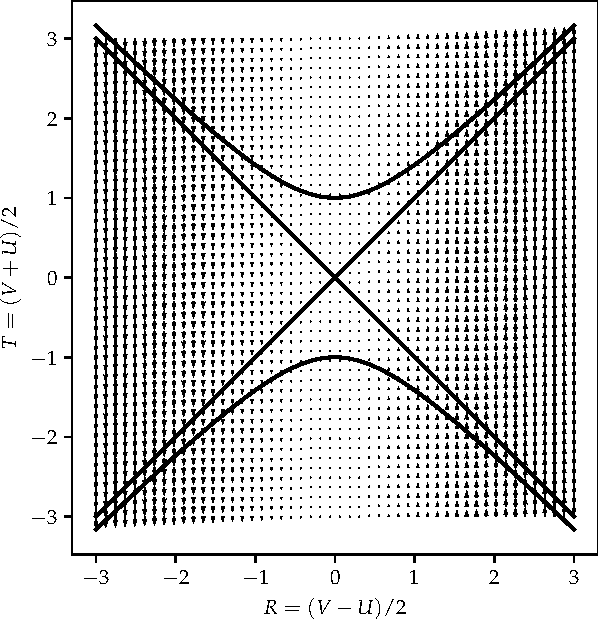
\includegraphics[width=.8\textwidth]{figures/killing_kruskal}
\caption{The vector field \(\xi \) shown in a Kruskal diagram.}
\label{fig:killing_kruskal}
\end{figure}

The metric reads %
\begin{align}
\mathrm{d} s^2 = - \frac{32 M^3}{r} \exp( - r/2M) \mathrm{d}U \mathrm{d}V + r^2 \mathrm{d}\Omega^2
\,.
\end{align}

Therefore, we can compute the norm of this Killing vector: it's 
%
\begin{align}
\xi^2 = 2\xi^U \xi^V g_{UV} = - \frac{32 M^3}{r} e^{-r/2M} (-UV) = 16 M^2 \left( \frac{2M}{r} - 1\right)
\,,
\end{align}
%
which is, up to a constant factor of \(16 M^2\), the same as the norm of the Killing vector \(\partial_t\) 
in regular Schwarzschild coordinates.
Since there is only one timelike Killing vector in the Schwarzschild exterior, 
the two must correspond to one another. Let us, however, show this explicitly.

The Kruskal coordinates relate to the regular Schwarzschild ones by %
\begin{align}
U = - \exp(- \frac{u}{4M}) \qquad \text{and} \qquad
V = \exp( \frac{v}{4M})
\,,
\end{align}
%
and %
\begin{align}
u = t - r - 2M \log (r/2M - 1) 
\qquad \text{and} \qquad
v = t + r + 2M \log (r/2M - 1) 
\,.
\end{align}

These relations allow us to also say that 
%
\begin{align}
UV = \left( 1 - \frac{r}{2M}\right) e^{r / 2M}
\qquad \text{and} \qquad
\frac{U}{V} = \exp(- \frac{t}{4M})
\,.
\end{align}

% We want to show that \(\xi \) is indeed a Killing vector. 

In order to transform \(\xi\) into Schwarzschild coordinates, we need the basis vectors: %
\begin{align}
\partial_U = \pdv{t}{U} \partial_t + \pdv{r}{U} \partial_r
\,,
\end{align}
%
and the calculation for \(V\) is analogous, with some opposite signs: 
let's do both at the same time, calling \(\chi \) either \(U\) or \(V\). 
The upper symbol in \(\pm\) and \(\mp\) corresponds to \(U\). 

The derivatives to compute (actually their inverses, since it's easier to work with these) are 
%
\begin{align}
\pdv{\chi }{r} &= \pdv{}{r} \left( \mp \exp( \mp  \frac{t \mp r \mp 2M \log (r / 2M - 1)}{4M})\right)  \\
&= \chi \pdv{}{r} \left(\frac{\mp t + r }{4M} + \frac{1}{2} \log ( \frac{r}{2M}- 1)\right)  \\
&= \chi \left( + \frac{1}{4M} + \frac{1}{(r / 2M - 1)} \frac{1}{(4M)}\right)  \\
&= + \frac{\chi}{4M} \left(\frac{r / 2M - 2}{r / 2M - 1} \right)
\,
\end{align}
%
and 
%
\begin{align}
\pdv{\chi }{t} &= \pdv{}{t} \left( \mp \exp( \mp  \frac{t \mp r \mp 2M \log (r / 2M - 1)}{4M})\right)  \\
&= \chi \pdv{}{t} \left(\frac{\mp t + r }{4M} + \frac{1}{2} \log ( \frac{r}{2M}- 1)\right)  \\
&= \mp \frac{\chi}{4M} 
\,.
\end{align}

Now we can go about writing down \(\xi\) in terms of Schwarzschild coordinates: %
\begin{align}
\xi &= - U \partial_U + V \partial_V  \\
&= - U \left(  \frac{4M}{U} \left( \frac{r - 2M}{r - 4M}\right)\partial_r - \frac{4M}{U} \partial_t \right)
+ V \left( \frac{4M}{V} \left( \frac{r - 2M}{r - 4M}\right)\partial_r + \frac{4M}{V} \partial_t \right)  \\
&= 8M \partial_t
\,.
\end{align}

We also recover the normalization: now, we can see that \(\xi^2 = \xi^t \xi^t g_{tt} = - 64M^2 (1 - 2M/r)\).

\todo[inline]{Wait! Why is it 64 here and 16 before?!}

A vector field \(\xi\) is a Killing vector field if \(\mathscr{L}_\xi g_{ab} = 0\), let's show this in \(U\), \(V\) coordinates: %
\begin{align}
\mathscr{L}_\xi g_{ab} &= 
\xi^c \partial_c g_{ab} 
+ g_{cb} \partial_a \xi^c
+ g_{ac} \partial_b \xi^c  \\
&= -U \partial_U g_{ab} + V \partial_V g_{ab} 
- g_{Ub} \partial_a U
+ g_{Vb} \partial_a V
- g_{aU} \partial_b U
+ g_{aV} \partial_b V
\,.
\end{align}

The only components which could be nonvanishing are those where either \(a\) or \(b\) equal \(U\) or \(V\). 

If \(a = b = U\), we only have the terms \(g_{Vb} \partial_a V + g_{aV} \partial_b V = 0\), and a similar thing happens with \(a = b = V\). 
By symmetry, the only other case is \(a = U\) and \(b = V\). We then get %
\begin{align}
\mathscr{L}_\xi g_{UV} &= - U \partial_U g_{UV} + V \partial_V g_{UV}
- g_{UV} \partial_U U
+ g_{UV} \partial_V V  \\
&= - U \partial_U g_{UV} + V \partial_V g_{UV}
\,.
\end{align}

We know that \(g_{UV}\) only depends on \(U\) and \(V\) through \(r\), and \(r\) only depends on \(UV\), so we will have %
\begin{align}
\mathscr{L}_\xi g_{UV} = 
- U \pdv{r}{U} \partial_r g_{UV} 
+ V \pdv{r}{V} \partial_r g_{UV} = (UV - VU) \partial_r g_{UV} = 0
\,.
\end{align}

\todo[inline]{I'd say that \(\xi\) is hypersurface-orthogonal, since it's just a rescaled \(\partial_t\), but maybe there's something more going on here?}

\subsection{Exercise 3}

Done in class.

\subsection{Exercise 4}

Alice is massive (no body shaming intended), therefore her trajectory will have a four-velocity \(u^a\) with \(u^2 = -1\). 

In Eddingston-Finkelstein coordinates, since the metric is 
%
\begin{align}
\dd{s^2} = - \left(1 - \frac{2M}{r} \right) \dd{v^2} + 2 \dd{v} \dd{r} + r^2 \dd{\Omega^2}
\,,
\end{align}
%
with \(v = t + r + 2 M \log(r / 2M - 1)\), this relation reads 
%
\begin{align}
-1 = - \left(1 - \frac{2M}{r}\right) \dot{v}^2 + 2 \dot{v} \dot{r}
\,,
\end{align}
%
where \(\dot{v}\) and \(\dot{r}\) are derivatives with respect to proper time, and we are using the assumption of radial motion together with spherical symmetry to see that \(\dot{\theta} = \dot{\varphi} = 0\) at all times.

A conserved quantity throughout this motion will be \(e = - \xi \cdot u\), since \(\xi = \partial_v\) is a Killing vector.\footnote{It is because we are just transforming \(\partial_t = (\pdv*{v}{t}) \partial_v = \partial_v\).} 
This reads %
\begin{align}
e = - \xi^v g_{vv} u^v - \xi^v g_{vr} u^r = \left(1 - \frac{2M}{r}\right) \dot{v} - \dot{r}
\,.
\end{align}


Using this, we can write the normalization of the four-velocity as %
\begin{align}
-1 &= -\dot{v} \left( \left(1 - \frac{2M}{r}\right) \dot{v} - 2 \dot{r}\right) = - \dot{v} \left( e  - \dot{r}\right)  \\
1 &= \dot{v} (e - \dot{r}) = \frac{e + \dot{r}}{1 - 2M / r} (e - \dot{r}) = \frac{e^2 - \dot{r}^2}{1 - 2M / r}  \\
1 - \frac{2M}{r} &= e^2 - \dot{r}^2 
\,.
\end{align}


This also helps us in computing the value of \(e\): we can simply evaluate this expression at the starting point \(r_0 = 4M\), since we know that there \(\dot{r} = 0\): \(e = \sqrt{1 - 2M / r_0} = 1/\sqrt{2}\).

We get an expression for \(r\) with a \(\pm\) ambiguity, but since we're describing infall we will select %
\begin{align}
\dot{r} = - \sqrt{ e^2 + \frac{2M}{r} -1 }
\,.
\end{align}

We can integrate this relation to compute the proper time required to go from \(r=4M\) to \(r= 2M\) or \(r=0\): %
\begin{align}
\tau_{4 \to 2} &= \int_{4M}^{2M} \dv{\tau }{r} \dd{r}  \\
&= \int_{2M}^{4M} \left(e^2 + \frac{2M}{r} - 1\right)^{-1/2} \dd{r}  \\
&= M \int_{2}^{4} \left(\frac{2}{\widetilde{r}} - \frac{1}{2}\right)^{-1/2} \dd{\widetilde{r}} \approx 7.3 M
\,.
\end{align}

The integrand is perfectly regular at \(\widetilde{r} = r / M = 2\) and \(\widetilde{r} = 0\), but it diverges at \(\widetilde{r} = 4\), since it is \(\sqrt{2 \widetilde{r} / (4-\widetilde{r})}\). 

However, this divergence is as \(x^{-1/2}\), where \(x = 4 - \widetilde{r}\), which has a finite integral.
This divergence is due to the initial condition we have set, \(\dot{r} = 0\) at \(r = 4M\). 

The calculation to go to \(r = 0\) is identical, and yields \(\tau _{4 \to 0} \approx 8.9 M\).

If, instead, we want to compute the coordinate time \(v_{4 \to 2}\) or \(v_{4 \to 0}\), we have to insert an extra ``conversion factor'' \(\dot{v}\) into the integral: %
\begin{align}
v_{4 \to 2} &= \int_{4M}^{2M} \dv{v}{\tau } \dv{\tau }{r} \dd{r}  \\
&= 
\int_{2M}^{4M} \frac{\dot{v}}{\dot{r}} \dd{r} = 
\int_{2M}^{4M} \frac{1}{\dot{r}(e - \dot{r})} \dd{r}  \\
&= M \int _2^4 \left( \sqrt{ \frac{2}{\widetilde{r}} - \frac{1}{2}} \left( \frac{1}{\sqrt{2}} + \sqrt{ \frac{2}{\widetilde{r}} - \frac{1}{2}}\right)  \right)^{-1} \dd{\widetilde{r}} \approx 7.7M
\,,
\end{align}
%
and similarly for \(v_{4 \to 0} \approx 8.6M\).

\begin{figure}[ht]
\centering
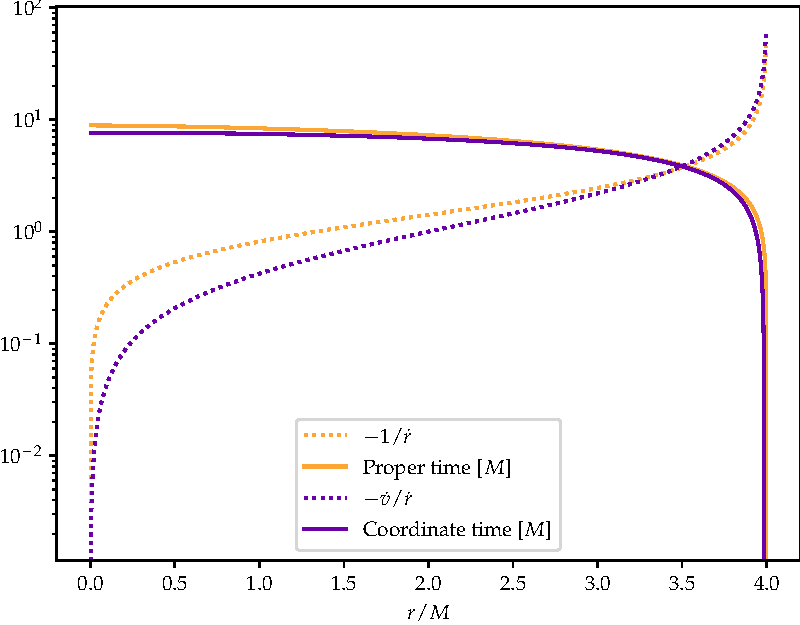
\includegraphics[width=.7\textwidth]{figures/ef_infall}
\caption{The filled lines correspond to the time for an observer to fall to the given radius starting from \(r = 4M\). The dashed lines are the corresponding integrands.}
\label{fig:ef_infall}
\end{figure}

\begin{figure}[ht]
\centering
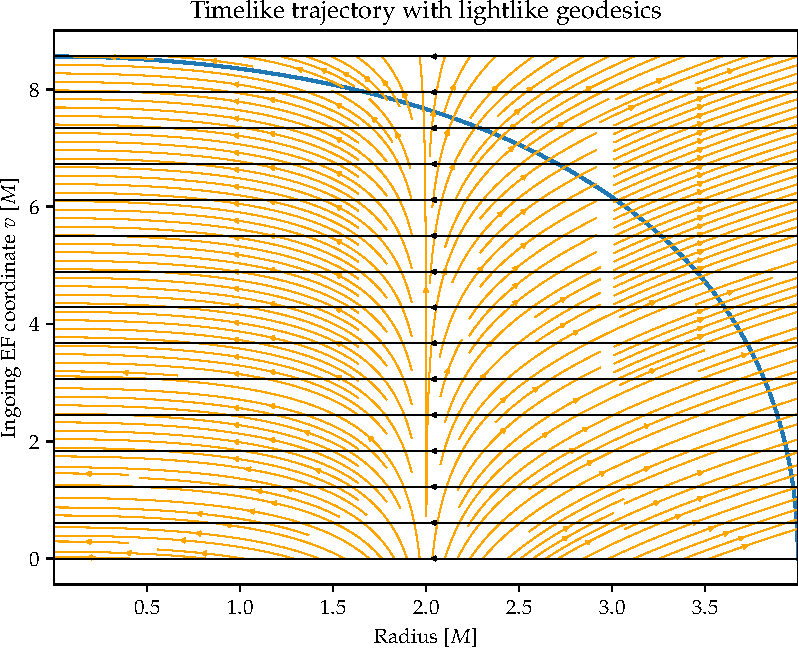
\includegraphics[width=\textwidth]{figures/spacetime_ef}
\caption{The geodesic infall of Alice, compared against lightlike geodesics.}
\label{fig:spacetime_ef}
\end{figure}

\subsection{Exercise 5}

We are looking at a FLRW metric \(\dd{s^2} = - \dd{t^2} + a^2(t) \dd{\Sigma^2}\), where \(a = \sqrt{ t / \alpha }\): a radiation-dominated universe. 
The Ricci scalar reads %
\begin{align}
R = 6 \left( \frac{\ddot{a}}{a} + \frac{\dot{a}^2}{a^2}\right)
\,,
\end{align}
%
and since \(\dot{a} = 1 / 2 \sqrt{t \alpha }\) and \(\ddot{a} = - 1 / 4 \sqrt{\alpha t^3}\) we will have \(R \propto t^{-2}\), which diverges as \(t \to 0\). This is sufficient to show that the spacetime is singular: it is not geodesically complete in the past.

\subsection{Exercise 6}

I already did this exercise, so here's the solution: the critical angle is 
%
\begin{align}
\alpha = \arcsin \sqrt{\frac{27M}{r} \left(1 - \frac{2M}{r}\right)}
\,.
\end{align}

The procedure is as follows: one can write out an equation in which the only quantities appearing are \(\dot{r}\) (derivative of \(r\) with respect to the affine parameter \(\lambda \)) and the two integrals of motion \(e = -u \cdot \partial_t\) and \(l = u \cdot \partial_\varphi \). 

This is in the form of a kinetic term plus a potential \(V _{\text{eff}}\), and the total ``effective energy'' depends on \(l\) and \(e\): \(E = e^2 / l^2\). 
The potential has a maximum at \(r= 3M\), \(V _{\text{max}} = 1/ 27 M^2\), so if starting at \(r < 3M\) the photon must overcome a potential barrier to get out.

So, all that's left is to relate \(l\) and \(e\) to the emission angle \(\alpha \). 

By performing a frame transformation, we find that %
\begin{align}
l = r \sin \alpha \qquad \text{and} \qquad
e = \sqrt{1 - 2M / r}
\,,
\end{align}
%
where the angle is interpreted as that which would be measured by a Schwarzchild-stationary observer.

\end{document}